\chapter{Julia}

Julia es un lenguaje de programación gratis cuyo propósito general es ser tan rápido como C, pero manteniendo la facilidad de lenguaje de R o Python. Es una combinación de sintaxis simple con alto rendimiento computacional. Su slogan es "Julia se ve como Python, se siente como Lisp, corre como Fortran" \citep{Hackers}. 
Esta combinación de características hace que Julia sea un lenguaje de programación que ha tomado mucha fuerza en la comunidad científica. Por lo tanto, en esta sección explicaré los básicos de Julia, desde su instalación hasta análisis de regresiones multivariadas. 

\section{Reproducibilidad}
Antes de empezar, es necesario enfatizar que esta tesis es completamente reproducible.En Peng y Hicks definen que "un análisis de datos publicado es reproducible si el conjunto de datos y el código utilizados para crear el análisis de datos está disponible para que otros lo analicen y estudien de manera independiente" \cite{peng2021reproducible}. A pesar de que en el artículo enfatizan que esta definición puede ser un poco ambigua, sí resaltan que la reproducibilidad es un medio para confiar y revisar el análisis de otros. Por lo tanto, en esta tesis decidí publicar el código que utilicé por medio de GITHUB y siempre hago énfasis en las fuentes de los datos. A pesar de que esta tesis no es un manual de Julia, Python o R considero da suma importancia publicar mi trabajo para que les sirva a mis compañeros ya sea como referencia o como punto de partida. 


\section{Instalación}
Al momento de escritura de esta tesis la versión de Julia disponible es la v1.6.3 hasta el 23 de Septiembre del 2021. Para descargar Julia, hay que entrar al siguiente link: \url{https://julialang.org/downloads/}. 

\subsection{Windows}
Para esta versión de Julia, las opciones disponibles de descarga son un instalador de 64-bits o uno de 32-bits. Para saber el tipo de Sistema que tiene tu ordenador de Windows, debes seleccionar el botón de \textsf{Start}, después \textsf{Configuración} $>$ \textsf{Sistema} $>$ \textsf{Acerca de}. En esta opción puedes ver el tipo de sistema que tiene tu computadora. Con esta información, eliges el instalador para tu computadora. Es importante seleccionar el \textsf{installer} y no el \textsf{portable}. Una vez descargado, seleccionas el archivo \textsf{.exe} y sigues los pasos de instalación. 


\subsection{Mac}
\valinline{No voy a abarcar tanto MAC porque no tengo Mac jaja}
Para el sistema operativo de Mac, solo hay una versión disponible de descarga. Selecciona la opción de 64-bit. Una vez descargado, mueve el archivo de Julia al folder de \textquotedblleft Aplicaciones\textquotedblright. Para verificar que está bien descargado, haz click en el ícono de Julia y debe salir una terminal como la siguiente: \val{Puedo copiar una imagen que no sea mía, sino de una página web? referenciendola obvio}


\section{Atom}
Atom es un editor de texto de programación. Su meta es \textit{no dificultar su uso ni posibilidad de modificación} \citep{ATOM}. \val{No estoy segura de como arreglar esto pero igual parece que no usaremos ATOM} Busca ser lo suficientemente fácil para que cualquier persona, ya sea principiante o experto en programación lo pueda utilizar. Por lo tanto, es una buena herramienta para escribir, editar y documentar el trabajo que uno hace en Julia. 

\subsection{Instalación en Windows} 
Por supuesto, el primer paso es instalar el programa. Para hacerlo, hay que ir a la página \url{https://atom.io/} y hacer clic en el botón de \textsf{Download}. 

Una vez descargado el archivo ejecutable solo hay que darle clic. Este proceso puede tardar un par de minutos. Sin embargo, una vez que termine el programa se ejecutará de manera automática. La pantalla se inicio se ve de la siguiente manera:

\begin{figure}[h]
\begin{center}
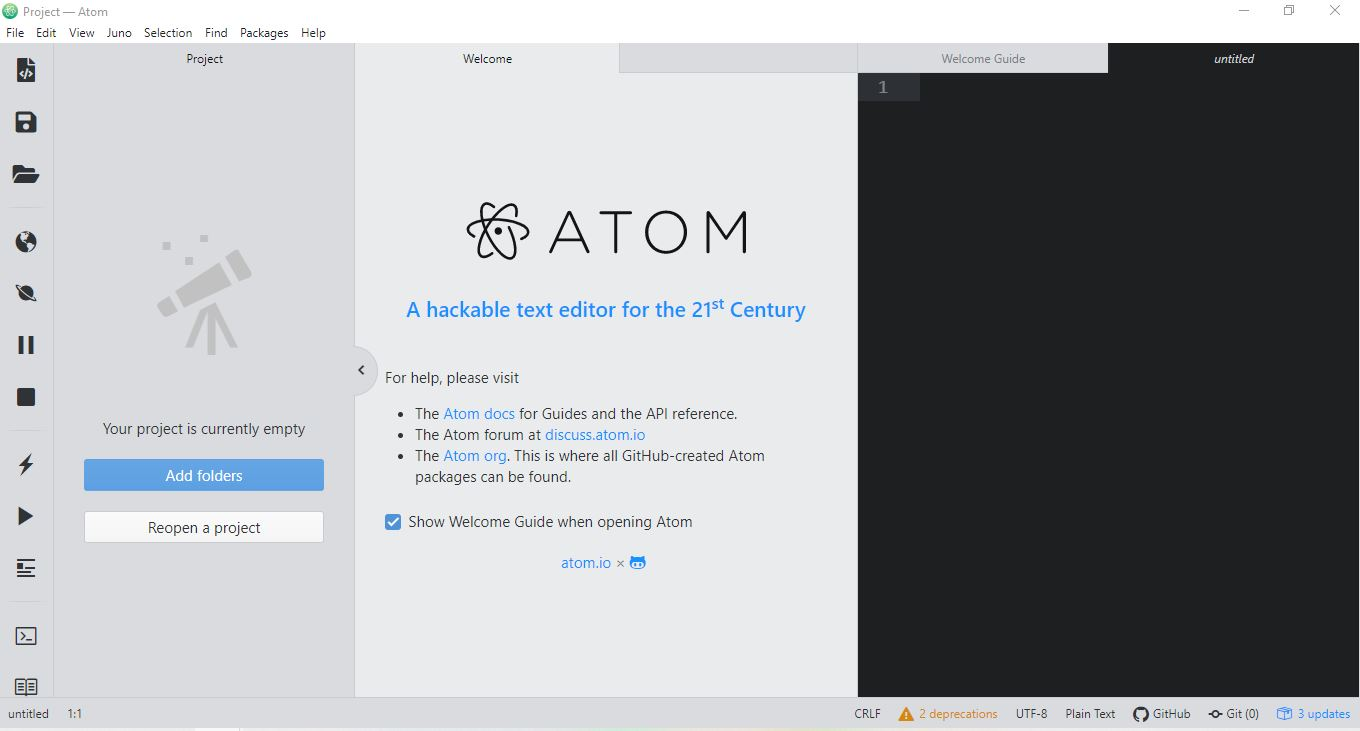
\includegraphics[scale=0.45]{Imagenes/atom_main_window.JPG}
 \caption{Ventana principal de Atom}
  \label{main_atom}
\end{center}
\end{figure}

El usuario puede modificar la pantalla de Atom con diferentes colores y temas siguiendo las instrucciones que vienen en la página \url{https://flight-manual.atom.io/getting-started/sections/atom-basics/}. Sin embargo, esa información no es relevante para esta tesis por lo que se va a omitir. 


\subsection{Conexión con Julia}
Ahora es momento de enlazar Julia con Atom. Para hacer esto, es necesario instalar el paquete Juno. 

\begin{enumerate}
    \item Abre Atom y selecciona \textsf{File} seguido de \textsf{Settings}. 
    \item En el panel izquierdo selecciona la opcion de \textsf{Install} y en el buscador de \textsf{Install Packages} escribe \textit{uber-juno}.
    \item Asegurate de que sea el paquete generado por JunoLab y haz click en el botón de \textsf{Install}. 
\end{enumerate}

Una vez instalado Juno, va a aparecer una opción llamada \textsf{Juno} en la parte superior de opciones entre \textsf{View} y \textsf{Selection}. Para correr Julia dentro de Atom debes seleccionar \textsf{Juno} y después \textsf{Open REPL}. Aparecerá una nueva ventana en la parte inferior de la pantalla que te dirá que oprimas enter para iniciar una sesión de Julia. Después de hacerlo, Julia iniciará y podrás usarlo de manera normal. 
\\
Una ventaja de Atom es utilizarlo por su función principal: ser un editor de texto de programación. Es una forma fácil y rápida de crear código de Julia y el usuario puede decidir si correrlo dentro de Atom o directo en Julia. Para crear un nuevo archivo, hay que seleccionar la opción de \textsf{File} en la parte superior izquierda y después la opción de \textsf{New File}. Para que Atom reconozca ese archivo como texto del lenguaje Julia hay que guardarlo con el nombre deseado agregando \texttt{.jl} al final del nombre. 



\section{Símbolo del sistema}
Otra opción (mi favorita) es correr Julia desde el símbolo del sistema (también conocido como \textit{Command Prompt} o cmd). De ahora en adelante, se usarán por igual los términos símbolo del sistema y cmd. Para facilitar el uso y trabajo en Julia, recomiendo agregar Julia a un \textit{PATH}. Las instrucciones para hacerlo en Windows 10 están en la página \url{https://julialang.org/downloads/platform/#windows}.

\subsection{\textit{Multithreading}}
Una de las razones por las que Julia es un lenguaje de programación muy rápido es que tiene la capacidad para multihilo (\textit{multithreading} en inglés). Esto significa que puede correr diferentes tareas de manera simultánea en varios hilos. De la manera más simple: la meta de los autores de Julia fue hacer un lenguaje de programación con un rendimiento tan alto que pudiera hacer varias cosas a la vez. Debido a que uno de los objetivos de esta tesis es medir la eficiencia y velocidad de Julia, es crucial conocer la característica del \textit{multithreading} y como utilizarla. 
\\
Juno automáticamente pone la misma cantidad de hilos que la cantidad de núcleos de procesadores disponibles \citep{multithreading-julia}. Sin embargo, esto se puede modificar entrando a \textsf{File} $>$ \textsf{Settings} $>$ \textsf{Packages}. Después, buscar el paquete \textit{julia-client} y seleccionar los \textsf{Settings} del paquete. Finalmente, dentro del apartado de \textsf{Julia Options} buscar \textsf{Number of Threads} y poner el número deseado. 
\\
Por otro lado, si se está usando el símbolo de sistema el camino es diferente. Antes de ejecutar julia, es necesario modificar la cantidad de hilos que se van a utilizar. En Windows, esto se hace escribiendo \texttt{set JULIA\_ NUM\_ THREADS=4} \citep{Julia_manual} En este ejemplo, se cambiaron los hilos a 4, pero se puede poner cualquier número. Sin embargo, se recomienda que el número no exceda de la cantidad de procesadores físicos de la computadora. Después de hacer esta modificación, ahora sí podemos ejecutar Julia. 
\\
Para observar que el cambio se ejecutó de manera correcta (en cualquiera de las dos opciones) basta con correr el comando \texttt{Threads.nthreads()} y observar que la respuesta sea el número deseado. 

\section{Jupyter}
Otra forma de correr Julia es utilizando Jupyther. Jupyter es un programa que exite para desarrollar software de manera pública en decenas de lenguajes de programación \val{Viene de la página oficial de Jupyter que todavía no tengo referencia}. Una de las ventajas de utilizar Jupyter para esta tesis es que se pueden utilizar los tres lenguajes de programación (R, Python y Julia) en un mismo software. 
\\
La manera más fácil para obtener Jupyter es instalanda Anaconda. Anaconda es ua interfaz gráfica que permite manejar y administrar aplicaciones, paquetes, ambientes y canales sin necesidad de usar comandos en el cmd. Para instalar Anaconda en Windows hay que ir a esta página \url{https://docs.anaconda.com/anaconda/install/windows/} y seguir las instrucciones de instalación. La instalación de este programa puede tomar unos cuantos minutos. 
\\
Una vez instalado Anaconda, basta con ejecutarlo y después seleccionar \textsf{Launch} debajo del ícono de Jupyter Notebook. Se abrirá una ventana en tu navegador como la siguiente: 

\begin{figure}[h]
\begin{center}
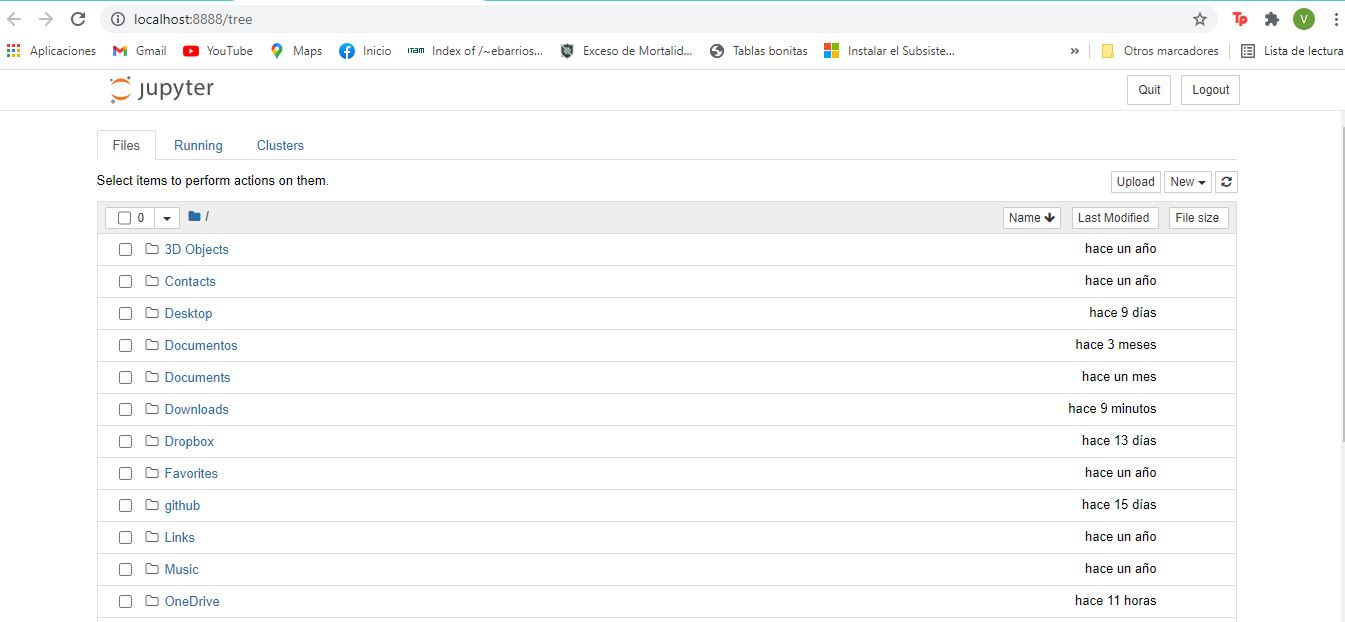
\includegraphics[scale=0.45]{Imagenes/inicio_jupyther.JPG}
 \caption{Ventana inicial de Jupyter}
  \label{main_jupyter}
\end{center}
\end{figure}

Para poder trabajar con Julia en Jupyter, hay que instalar el paquete \texttt{IJulia} como en las instrucciones % \ref{instalacion_paquete}.

\valinline{No me gustaría agregar en esta parte la instalación de paquetes pero si se tiene que hacer pues ni modo} 
Para confirmar que la instalación está bien hecha hay que abrir Jupyter, seleccionar \textsf{New} y debe aparecer la opción de \textsf{Julia 1.6.3}.


\section{Básicos de Julia}
Como ya se mencionó, Julia busca ser un lenguaje de programación sencillo e intuitivo. Por lo tanto, su sintáxis es bastante sencilla. La asignación de variables se hace con un signo de igualdad $=$. El ejemplo más sencillo de esto sería \texttt{x = 2} donde denotamos a x el valor de 2. Toda la información sobre la sintaxis que utiliza Julia viene del manual oficial de Julia \citep{Julia_manual}.

\subsection{Operaciones básicas}
La siguiente tabla muestra la sintaxis usada para las operaciones básicas en Julia. 
\\

\begin{tabular}{|c|c|c|}
\hline 
\rule[-1ex]{0pt}{2.5ex} Expresión & Nombre & Descripción \\ 
\hline 
\rule[-1ex]{0pt}{2.5ex} \texttt{+x} & suma unaria & la operación identidad \\ 
\hline 
\rule[-1ex]{0pt}{2.5ex} \texttt{-x} & resta unaria & asigna a los valores sus inversos aditivos \\ 
\hline 
\rule[-1ex]{0pt}{2.5ex} \texttt{x + y} & suma binaria & realiza adición \\ 
\hline 
\rule[-1ex]{0pt}{2.5ex} \texttt{x - y} & resta binaria & realiza sustracción \\
\hline 
\rule[-1ex]{0pt}{2.5ex} \texttt{x * y} & multiplicación & realiza multiplicación \\
\hline 
\rule[-1ex]{0pt}{2.5ex} \texttt{x / y} & división & realiza divisiones \\
\hline 
\rule[-1ex]{0pt}{2.5ex} \texttt{x $\div$ y} & división de enteros & $x / y$ truncado a un entero \\
\hline 
\rule[-1ex]{0pt}{2.5ex} \texttt{x $\setminus$ y} & división inversa & equivalente a dividir \texttt{y / x} \\
\hline 
\rule[-1ex]{0pt}{2.5ex} \texttt{x $\wedge$ y} & potencia & eleva \texttt{x} a la potencia \texttt{y} \\
\hline 
\rule[-1ex]{0pt}{2.5ex} \texttt{x \% y} & residuo & equivalente a \texttt{rem(x,y)} \\
\hline 
\end{tabular} 

La siguiente tabla muestra los operadores booleanos en Julia. \val{Se ven horribles los \& \& pero ncon verbatim no funciona}

\begin{center}
\begin{tabular}{ |c|c| } 
 \hline
 $!x$ & negación \\ 
 $x$ \& \& $y$ & operador de circuito corto $and$ \\ 
 $x \parallel y$ & operador de circuito corto $or$ \\ 
 \hline
\end{tabular}
\end{center}

\subsubsection{Operaciones básicas en vectores}
En Julia, para cada operación binaria existe su correspondiente operación punto (\textit{dot operation} en inglés). Estas funciones están definidas para efectuarse elemento por elemento en vectores y matrices. Para llamarse, basta agregar un punto antes del operador binario. Por ejemplo,
 \texttt{[1 9 9 7] .$\wedge$ 2} eleva cada uno de los elementos del vector al cuadrado. 
\\
También es importante mencionar que Julia maneja los números imaginarios utilizando el sufijo \texttt{im}. Sin embargo, como no utilizaran en esta tesis, se omitirá mayor explicacion. 


\subsection{\textit{Strings} (secuencias de caracteres)} 

Además de números, Julia puede asignar characteres a variables. Esto se hace utilizando las comillas dobles. Por ejemplo,

\begin{minted}{julia}
    string = "Esta tesis es genial"
\end{minted}


\begin{tcolorbox}
      \texttt{Esta tesis es genial}
\end{tcolorbox}

Similar a otros lenguajes de programación, podemos accesar a caracteres específicos de un string utilizando corchetes cuadrados $[$ $]$ y a cadenas seguidas de caracteres usando dos puntos $:$. Continuando con el ejemplo anterior, 

\valinline{Como pongo esto que se vean los resultados?}
\begin{figure}[h]
\begin{center}
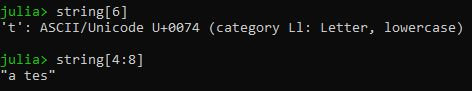
\includegraphics[scale=0.8]{Imagenes/ejemplo_string_partes.JPG}
  \label{ejemplo_string_julia_partes}
\end{center}
\end{figure}

Además, Julia también cuenta con la opción de concatenación de múltiples strings. Esto se hace utilizando un asterisco $*$ para separar cada uno de los strings. Por ejemplo,

\begin{figure}[H]
\begin{center}
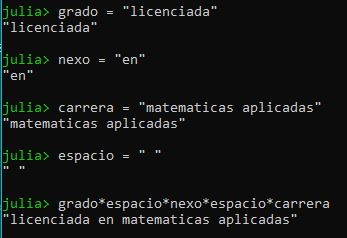
\includegraphics[scale=0.8]{Imagenes/ejemplo_concatenacion.JPG}
  \label{ejemplo_string_concatenacion}
\end{center}
\end{figure}

\subsection{Funciones}
En Julia, una función es un objeto que asigna una tupla de argumentos a un valor de retorno \citep{Julia_manual}. La sintáxis básica para definir funciones en Julia es:

\begin{figure}[h]
\begin{center}
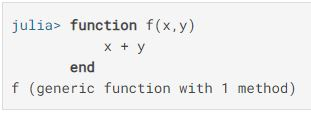
\includegraphics[scale=0.6]{Imagenes/sintaxis_funcion.JPG}
 \caption{Sintáxis básica de una función en Julia.}
  \label{functions_sintax_Julia}
\end{center}
\end{figure}

Además, puedes agregar la palabra \textit{return} para que la función regrese un valor. Por ejemplo, si quisieramos tener una función a la que le des dos números y te regrese el número mayor, la función sería la siguiente:

\begin{tcolorbox}
      \begin{verbatim}
          function numero_mayor(x, y)
              if (x > y)
                  return x 
              else
                  return y
              end
         end
      \end{verbatim}
\end{tcolorbox}


Para llamar a la función bastaría con escribir \texttt{numero\_mayor(x, y)} asignando o sustituyendo valores por $x$ y $y$. 

\subsection{Vectores y Matrices}

\begin{definition}
Un vector columna de $n$ componentes se define como un conjunto ordenado de $n$ números escritos de la siguiente manera:
\begin{equation*}
    \begin{aligned}
    \begin{pmatrix}
    x_1 \\ 
    x_2 \\
    \vdots \\
    x_n
    \end{pmatrix} 
    \end{aligned}
\end{equation*}
\end{definition}


En Julia, para definir un vector columna se hace uso de los corchetes cuadrados $[$ $]$ y comas. Por ejemplo, 

\begin{figure}[h]
\begin{center}
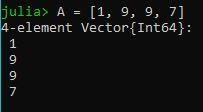
\includegraphics[scale=0.8]{Imagenes/vector_columna_julia.JPG}
  \label{vector_columna}
\end{center}
\end{figure}

\begin{tcolorbox}
      \begin{verbatim}
         A = [1, 9, 9, 7]
      \end{verbatim}
\end{tcolorbox}
da como resultado un vector de 4 elementos de tipo Int64. \val{Me interesa mucho ver lo de los tipos}

Si quisiera definir un vector renglón, se hace exactamente igual solamente omitiendo el uso de las comas. Sin embargo, es importante señalar que  ahora Julia tomó el objeto A como una matriz, no como un vector. 

\begin{definition}
Una matriz $A$ de $m \times n$ es un arreglo rectangular de $mn$ números dispuestos en $m$ renglones y $n$ columnas. 

\begin{equation*}
    \begin{aligned}
    \begin{pmatrix}
    a_{11} & a_{12} & \dots & a_{1j} & \dots & a_{1n} \\
    a_{21} & a_{22} & \dots & a_{2j} & \dots & a_{2n} \\
    \vdots &  \vdots  &  \ddots &  \vdots  & \ddots &\vdots\\
    a_{i1} & a_{i2} & \dots & a_{ij} & \dots & a_{in} \\
    \vdots &  \vdots  &  \ddots &  \vdots  & \ddots &\vdots\\
     a_{m1} & a_{m2} & \dots & a_{mj} & \dots & a_{mn} \\
    \end{pmatrix} 
    \end{aligned}
\end{equation*}
\end{definition}


En Julia, hay dos formas de definir matrices. La primera es utilizando los corchetes cuadrados $[$ $]$ para comenzar y terminar la matriz. Las columnas están separadas por espacios y las filas por punto y coma. La segunda opción similar a la primera con la única diferencia de que en lugar de punto y coma se cambia de renglón. Esta opción puede ser un poco tediosa ya que requieren que las columnas estén alineadas. Sin embargo, es una forma más visual de ver las matrices. En la siguiente tabla se pueden ver ambas opciones. 

\begin{figure}[h]
\begin{center}
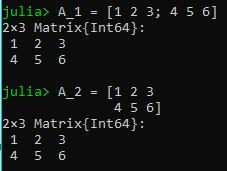
\includegraphics[scale=0.8]{Imagenes/definir_matrices.JPG}
  \label{definicion_matrices}
\end{center}
\end{figure}

\begin{tcolorbox}
      \begin{verbatim}
         A_1 = [1 2 3; 4 5 6]
         A_2 = [1 2 3 
                4 5 6]
      \end{verbatim}
\end{tcolorbox}

De manera análoga con los vectores, para llamar un solo elemento de la matriz se utilizan los corchetes cuadrados. Continuando con el ejemplo anterior, para obtener el número 5 de la matriz $\text{A\_2}$, se programaría el código $\texttt{A\_2[2, 2]}$.

\valinline{No estoy segura de si poner las operaciones básicas de matrices (con sus definiciones, claro) ni la concatenación de matrices}


\subsection{\textit{DataFrames}}
Ya que conocemos los arreglos básicos que se pueden manejar en Julia es momento de conocer y manejar los \textit{dataframes}. Un dataframe es una tabla estructurada de dos dimensiones que se usa para tabular distintos tipos de datos. Julia tiene un paquete llamado \textit{DataFrames}  que permite trabajar con dataframes que uno crea en Julia o que viene de alguna base de datos externa. 

\subsubsection{Instalación del paquete}
Similar a otros lenguajes de programación, cuando se usa un paquete por primera vez hay que instalarlo. En las ocasiones siguientes donde se quiera volver a usar el paquete basta con llamarlo con la palabra \texttt{using}. 
\\
Para instalar el paquete, hay que poner las siguientes líneas de código. 
\val{Lo malo de esta versión es que no encuentro como enumerarlo}

\begin{minted}{julia} 
     using Pkg
     Pkg.add("DataFrames")
     using DataFrames
\end{minted}


\begin{tcolorbox}
\begin{equation}
\begin{aligned} \label{instalacion_paquete}
       \texttt{using Pkg} \\
        \texttt{Pkg.add("DataFrames")} \\
        \texttt{using DataFrames}
\end{aligned}
\end{equation}
\end{tcolorbox}


La primera línea de comando le está diciendo a Julia que use el paquete llamado \texttt{Pkg}. Este paquete viene por default en la instalación de Julia. La segunda línea le está indicando a Julia que agregue el paquete llamado \texttt{DataFrames}. 
Una vez instalado el paquete de DataFrames, hay que hacerle saber a Julia que lo queremos usar en esta ocasión. Para eso, utilizamos la tercera línea del código. En caso de que Julia no marque ningún error, el paquete está listo para utilizarse. 

\subsubsection{Crear un dataframe}

Aunque de manera general los dataframes se utilicen para manejar grandes cantidades de información exportada de otros formatos, es importante saber como se crea y manipula un dataframe desde cero en Julia. Para crear un dataframe, hay que escribir la palabra \texttt{DataFrame} y abrir un paréntesis. Después, se escribe el nombre de la primera columna, un signo de igualdad y los datos que corresponden a esa variable. Se repite lo mismo con la cantidad de columnas que se requieran. Por ejemplo, para hacer un dataframe con las claves únicas y nombres de cinco mujeres el código sería el siguiente: 


\begin{tcolorbox}
    \begin{verbatim}
    df = DataFrame(id = 1:5, 
    nombre = ["Valeria", "Paula", "María José", 
        "Sofía", "Mónica"])
    \end{verbatim}
\end{tcolorbox}



Es importante nombrar las columnas del dataframe ya que de esta forma basta con escribir \texttt{df.col} para referirnos a la columna llamada col del dataframe llamado df. De la misma manera, si se quisiera agregar una columna nueva basta con asignarle datos a \texttt{df.colNueva}. Por ejemplo, si quisieramos agregar una columna llamada \texttt{color} al dataframe del ejemplo anterior, el código sería el siguiente: 

\begin{minted}{julia}
     df.color = ["morado", "azul", "verde", "negro", "rojo"]
\end{minted}

\begin{tcolorbox}
    \begin{verbatim}
    df.color = ["morado", "azul", "verde", 
        "negro", "rojo"]
    \end{verbatim}
\end{tcolorbox}


Como cualquier otro objeto en Julia, los dataframes tienen diferentes funciones como seleccionar un subgrupo de datos, agregar datos por renglones, modificar y eliminar datos, etc. Sin embargo, eso no es de relevancia para esta tesis por lo que se omitirá. 

\subsubsection{Importar datos en un dataframe}

Como se mencionó anteriormente, los dataframes son utilizados para contener grandes cantidades de información. Usualmente, esta información no es generada en Julia por lo que hay importarla. Una de las formas más rápidas es usando el paquete \texttt{CSV}. Para instalarlo, hay que seguir los pasos como en la  \ref{instalacion_paquete} cambiando \texttt{DataFrames} por \texttt{CSV}. 
\\
Una vez instalado el programa, basta utilizar el comando \texttt{CSV.read} y la ruta de la ubicación del archivo para exportar los datos. Por ejemplo, 

\begin{minted}{julia}
     df = CSV.read("C:/Users/Valeria/Documents/ITAM/Tesis/Julia con R/ejemplo.csv", DataFrame)
\end{minted}

\begin{figure}[h]
\begin{center}
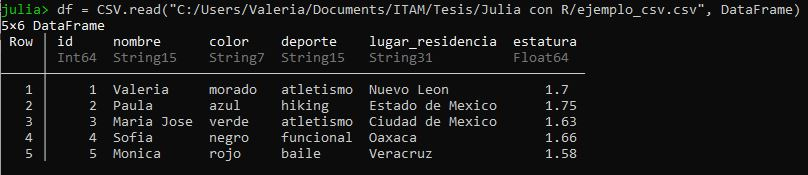
\includegraphics[scale=0.6]{Imagenes/insertar_df.JPG}
  \label{insertar_df}
\end{center}
\end{figure}

\subsection{Regresiones}

\valinline{Buen link de ayuda \url{https://www.machinelearningplus.com/linear-regression-in-julia/}}
Una vez que ya podemos manejar relativamente grandes volúmenes de información en un dataframe en Julia, podemos empezar con la parte verdaderamente estadística. ¿Cuál es el punto de tener una muestra de tamaño significativo si no sabemos analizarla? Una de las maravillas que nos regala la estadística es el uso de regresiones para intentar darle algún sentido o explicación a los datos. 


Regresión es un método que permite a los investigadores resumir como predicciones o valores promedio de un resultado varian a través de variables individuales definidas como predictores. \citep{regression_other_stories} 

En pocas palabras, una regresión es una fórmula que intenta explicar como una variable depende otras. Como es de esperarse, Julia tiene un paquete llamado \texttt{GLM} que calcula modelos lineales. Para instalarlo y utilizarlo, hay que seguir las instrucciones que vienen en la tabla \ref{instalacion_paquete} con este paquete. Para ajustar un modelo lineal generalizado, hay que usar la función \texttt{glm(formula, data, family, link)} donde 

\begin{itemize}
    \item \texttt{formula}: usa los nombres de las columnas del dataframe de datos para referirse a las variables predictoras
    \item \texttt{data}: el dataframe que contenga los predictores de las formula
    \item \texttt{family}: podemos elegir entre Bernoulli(), Binomial(), Gamma(), Normal(), Poisson() o NegativeBinomial() \val{Todavía no entiendo muy bien esto}
    \item \texttt{link}: \val{no entiendo muy bien a que se refiere esto, creo que está fuera del alcance de la tesis}
\end{itemize}

\valinline{Viene del manual de GLM que todavia no tengo referencia}

\subsubsection{Regresión lineal simple}
El modelo de regresión lineal más simple es el que tiene un solo predictor: 

\begin{equation}
    \begin{aligned}
    y = a + bx + \epsilon
    \end{aligned}
\end{equation}

Para este modelo, use los datos de \citep{regression_other_stories} sobre el modelo creado por Douglas Hibbs para predecir las elecciones de Estados Unidos basandose solamente en el crecimiento económico. Los datos se ven de la siguiente manera: \val{Como le hago para incluir esto?}

\begin{figure}[H]
\begin{center}
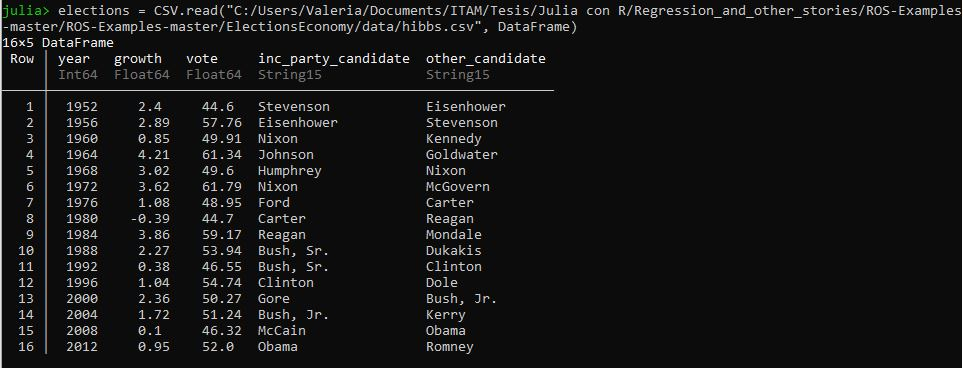
\includegraphics[scale=0.5]{Imagenes/elections_dataframe.JPG}
  \label{elections_dataframe}
\end{center}
\end{figure}

El modelo que buscamos es que el voto sea resultado del crecimiento económico. Por lo tanto, el modelo programdo en Julia se ve de la siguiente manera:

\begin{figure}[h]
\begin{center}
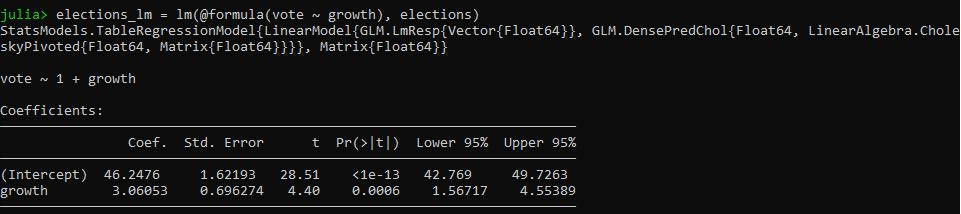
\includegraphics[scale=0.5]{Imagenes/elections_modelo.JPG}
  \label{elections_modelo}
\end{center}
\end{figure}

Al resultado de la regresión es el modelo $y = 46.3 + 3.1x$. \val{Solo para que quede claro, es lo mismo que viene en el libro de Gelman}


\subsubsection{Regresión lineal múltiple}

\valinline{Todo esto lo saque de \citep{regression_other_stories}}

El modelo de regresión lineal clásico para múltiples predictores es 

\begin{equation*}
    \begin{aligned}
    y_i = \beta_1 X_{i1} + \dots + \beta_k X_{ik} + \epsilon_i, \text{ para } i = 1, \dots, n
    \end{aligned}
\end{equation*}

donde los errores $\epsilon_i$ son independientes e idénticamente distribuidos de manera normal con media 0 y varianza $\sigma^2$. La representación matricial equivalente es 

\begin{equation*}
    \begin{aligned}
        y_i = X_i \beta + \epsilon_i, \text{ para } i = 1, \dots, n
    \end{aligned}
\end{equation*}

donde $X$ es una matriz de $n \times k$ con renglón $X_i$.
\\
En primer lugar, analicé un modelo que incluye una relación entre dos predictores. Para este modelo, usé los datos de \citep{regression_other_stories} sobre la relación entre los resultados de exámenes de niños (\texttt{kid\_score}), el coeficiente intelectual IQ de sus madres (\texttt{mom\_iq}) y si sus madres terminaron o no la preparatoria (\texttt{mom\_hs}). 
\\
La relación que intento modelar es si el coeficiente intelectual y la educación de las madres afectan los resultados de los exámenes de los niños. Por lo tanto, los predictores son las variables en relación con la madre mientras que la respuesta es el desempeño de los niños. El código en Julia se ve de la siguiente manera

\begin{minted}{julia}
    using DataFrames, GLM, CSV

    data_kid = CSV.read("C:/Users/Valeria/Documents/ITAM/Tesis/Julia con R/Regression_and_other_stories/ROS-Examples-master/ROS-Examples-master/KidIQ/data/kidiq.csv", DataFrame)

    fm = @formula(kid_score ~ mom_hs + mom_iq + mom_hs*mom_iq)

    kidscore_lm = lm(fm, data_kid)
\end{minted}

Lo cual da como resultado el modelo 

\valinline{OJO que el coeficiente de momiq sale en R como 1.1 y aquí como 0.97}

\begin{equation*}
    \begin{aligned}
        kid\_score = -11.48 + 51.26* mom\_hs + 0.97*mom\_iq -0.48*mom\_hs*mom\_iq + \epsilon
    \end{aligned}
\end{equation*}

Por lo tanto, para incluir la relación entre dos predictores, basta usar un asterisco entre ellos en la formula de la regresión. 
\\
\valinline{Me acabo de dar cuenta de eso del paquete CSV. Cambio todo para que ahora sea CSVFiles?? O solo lo menciono??}
Como segundo ejemplo, analicé un modelo que tiene una variable categórica para mostrar su aplicación en Julia. A diferencia de otros lenguajes, en Julia no hay que especificar si el predictor es una variable categórica. Sin embargo, si la base de datos tiene valores faltantes (\textit{missing values}) es mejor utilizar el paquete llamado \textsf{CSVFiles}. La instalación y uso del paquete es igual que como se muestra en las instrucciones \ref{instalacion_paquete}.  
\\
Tomando en cuenta lo anterior, utilicé datos de una encuesta hecha a 1816 personas que buscaba predecir sus ganancias anuales tomando en cuenta aspectos como su altura, peso, sexo, etnicidad, educación, educación de los padres, etc. Para este ejemplo en específico, los predictores son la altura centrada en el promedio (\texttt{cHeight}), el sexo (\texttt{male}) y la etnicidad (\texttt{ethnicity}). La variable respuesta es el peso (\texttt{weight}). La razón por la que se centró la altura es para mejorar la comprensión del modelo. El código en Julia para este modelo es el siguiente:

\begin{minted}{julia}
    using DataFrames, GLM, CSVFiles

    earnings_data = DataFrame(load("C:/Users/Valeria/Documents/ITAM/Tesis/Julia con R/Regression_and_other_stories/ROS-Examples-master/ROS-Examples-master/Earnings/data/earnings.csv"))
    earnings_data.cHeight = earnings_data.height .- 66

    fm = @formula(weight ~ cHeight + male + ethnicity)
    earnings_lm = lm(fm, earnings_data)

\end{minted}

El resultado es la regresión \val{Se ve bien así en tabla, no?}

\valinline{Otra vez, los resultados son levemente diferentes que en el libro}

\begin{tabular}{|c|c|c|}
    \hline 
    \rule[-1ex]{0pt}{2.5ex}  & Coeficiente & Error Estándar \\ 
    \hline 
    \rule[-1ex]{0pt}{2.5ex} \texttt{cHeight} & 154.33 & 2.23 \\
    \hline 
    \rule[-1ex]{0pt}{2.5ex} \texttt{male} & 3.85 & 0.25 \\ 
    \hline 
    \rule[-1ex]{0pt}{2.5ex} \texttt{ethnicity: Hispanic} & -6.15 & 3.56 \\ 
    \hline 
    \rule[-1ex]{0pt}{2.5ex} \texttt{ethnicity: Other} & -12.26 & 5.18 \\ 
    \hline 
    \rule[-1ex]{0pt}{2.5ex} \texttt{ethnicity: White} & -5.19 & 2.27 \\ 
    \hline
\end{tabular}





\subsubsection{Gráfica de resultados}

\subsubsection{Histograma}

\subsubsection{Gráfica cuantil-cuantil}

\subsubsection{Análisis de residuales}

\subsubsection{Tabla de análisis de varianza}


\subsection{Paquete Distributions}
Para aprender como funcionan las distribuciones en Julia. El manual del paquete viene aquí \url{https://juliastats.org/Distributions.jl/v0.14/index.html}




